\documentclass[UTF8]{ctexart}
\usepackage{ctex}
\usepackage{geometry}
\geometry{left=3.18cm,right=3.18cm,top=2.54cm,bottom=2.54cm}
\usepackage{graphicx}
\usepackage{framed}
\usepackage{fancyhdr}
\usepackage{setspace}
\pagestyle{fancy}%清除原页眉页脚样式
\fancyhf{}
\fancyhead[C]{华中科技大学电信学院}
\fancyfoot[C]{\thepage}
% \pagestyle{plain}
\begin{document}
\begin{center}
    \quad \\
    \quad \\
    % \kaishu \fontsize{35}{5} \textbf{华 中 科 技 大 学}
    % \vskip 3cm
    \fangsong \fontsize{49}{5}《通信电子线路》实验报告
    \vskip 3cm
    \heiti \zihao{1}\textbf{高频小信号}
    \fangsong \zihao{1} 放大器仿真
\end{center}

\makeatletter
\newcommand\dlmu[2][4cm]{\hskip1pt\underline{\hb@xt@ #1{\hss#2\hss}}\hskip3pt}
\makeatother

\vskip 3cm
\begin{center}
    \zihao{3}
    \begin{tabular}{rl}
         & \makebox[4em][s]{学生姓名}	\hspace{0.2cm}	\dlmu[9cm]{赵展}
         \\
         & \makebox[4em][s]{学号}	\hspace{0.2cm}	\dlmu[9cm]{U202117282}
         \\
         & \makebox[4em][s]{专业班级}	\hspace{0.2cm}		\dlmu[9cm]{种子2101班}
         \\
         & \makebox[4em][s]{实验平台}	\hspace{0.2cm}		\dlmu[9cm]{Multisim 14.3 on Windows}
         \\
    \end{tabular}
    \vskip 3cm
    2023年10月26日
\end{center}

\newpage
\tableofcontents
\newpage
\section{实验目的}
\begin{itemize}
    \item 熟悉NIMultisim 电路仿真软件的使用
    \item 学会使用NIMultisim仿真软件观察高频小信号放大电路的静态工作点
    \item 熟悉使用NIMUltisim仿真软件观察高频小信号放大电路的时域波形
    \item 熟悉使用NIMultisim仿真软件观察电路的幅频和相频响应
\end{itemize}
\section{实验内容}
\begin{itemize}
    \item 使用NIMultisim 绘制高频谐振小信号放大器的仿真电路,分析直流偏置工作点
    \item 进行时域仿真,观察时域波形
    \item 进行频域仿真,分析电路频域响应
    \item 验证品质因素QL、通频带B和电压增益AV0之间的关系
    \item 要求输入信号频率至少为10MHz
\end{itemize}
\section{实验原理}
已经知道高频小信号放大器的原理图如图\ref{img:small_signal_principle}所示,$R_1,R_2,R_3$为偏置电阻,$L_F,C_F$
为滤波电路,该电路采用负压供电,$C_4,L$组成LC谐振回路。$R_4$用于加宽回路频带,
略去支流参数后即可用Y参数等效电路进行模拟。
\begin{figure}[htbp]
    \centering
    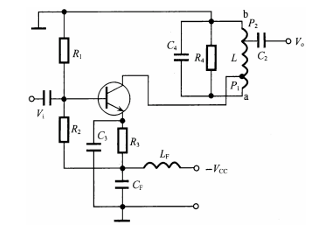
\includegraphics[width=0.8\linewidth]{small_signal_principle.png}
    \caption{高频小信号放大器原理图}
    \label{img:small_signal_principle}
\end{figure}
其对应的Y参数等效电路如图\ref{img:small_signal_principle_Y}所示
\begin{figure}[htbp]
    \centering
    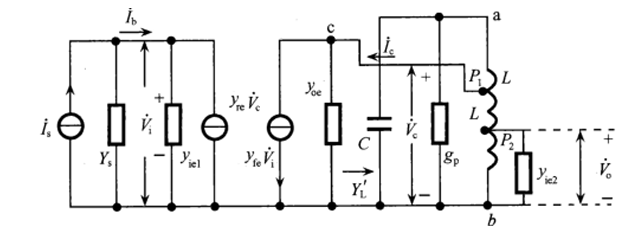
\includegraphics[width=0.8\linewidth]{small_signal_principle_Y.png}
    \caption{高频小信号放大器Y参数等效电路}
    \label{img:small_signal_principle_Y}
\end{figure}
根据Y参数等效电路可以得到谐振时公式:
$$
A_{V0}=-\frac{P_1 P_2 y_{ie}}{g_{\Sigma }+P_1^2 g_{oe}+P_2^2 g_{ie2}}
$$
根据高频小信号放大器原理图,在Multisim中搭建实验电路如图\ref{img:multisim_circuitry}所示
\begin{figure}[htbp]
    \centering
    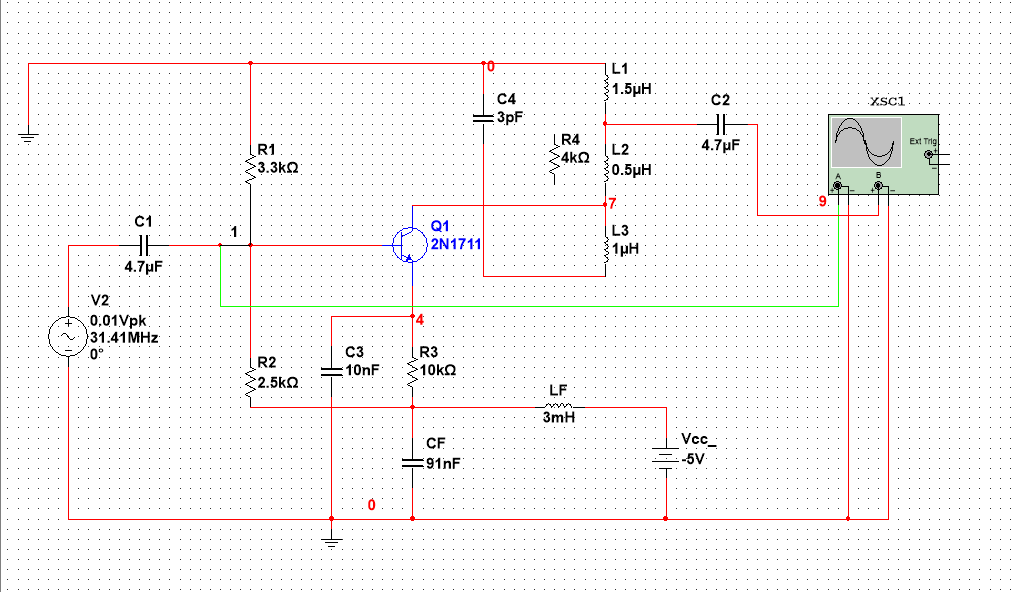
\includegraphics[width=0.8\linewidth]{multisim_circuitry.png}
    \caption{高频小信号放大器仿真电路}
    \label{img:multisim_circuitry}
\end{figure}
其中,使用三极管的型号为2N1711,发射极使用$4.7\mu F$电容耦合,输出端使用$4.7\mu F$电容滤
直流,使用三个电感来模拟电感抽头,$R_1,R_2$为基极提供直流偏置,示波器两个端口分别接
输入与输出端,其中绿色连接输入端;红色连接输出端。
\section{实验步骤}
\begin{enumerate}
    \item 按照实验原理图,搭建仿真实验电路
    \item 验证静态工作点
    \item 观察时域波形:启动仿真后,开启示波器,观察输入输出波形;使用瞬态分析,添加选频网络处电感/电容的电压作为观察量,启动仿真
    \item 观察频域特性:分别对输入输出信号使用傅里叶分析,观察其频谱图;使用交流分析,添加$A_V$为其观察量,得到幅频响应曲线与相频响应曲线,并标出其通频带
    \item 将$R_4$接上选频网络,重复第4步,比较增益,通频带,品质因数的变化
\end{enumerate}
\section{实验结果与分析}
\subsection{时域特性}
\subsubsection{输入输出信号波形}
根据以上的实验步骤,示波器中所得输入输出波形如图\ref{img:multisim_time_signal_graph}所示。
由示波器波形可知,输出电压$V_0$最大值约为85.870mV,输入电压最大值约为9.952mV,放大倍数为$|A_V|=\frac{85.870}{9.952}=8.628$。
\begin{figure}[htbp]
    \centering
    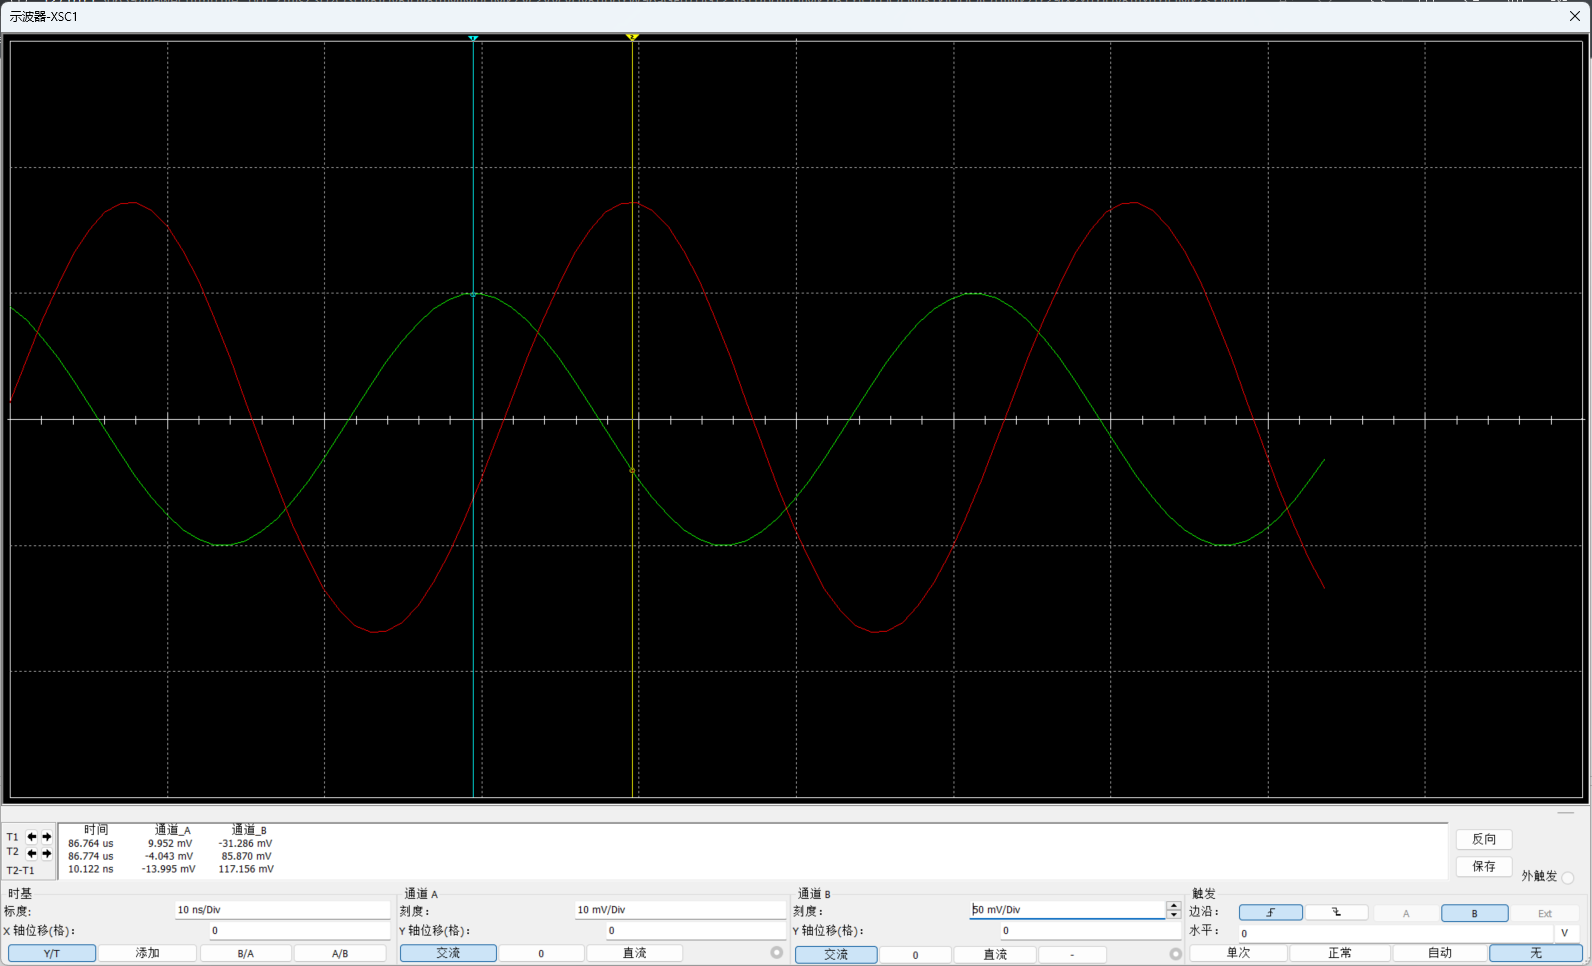
\includegraphics[width=0.8\linewidth]{multisim_time_signal_graph.png}
    \caption{示波器:输入输出波形}
    \label{img:multisim_time_signal_graph}
\end{figure}
\subsubsection{电感/电容电压}
在$L_3$与$C_4$的连接处添加探针,得到选频网络中电感/电容的电压仿真如图\ref{img:multisim_transient_analysis}所示.
\begin{figure}[htbp]
    \centering
    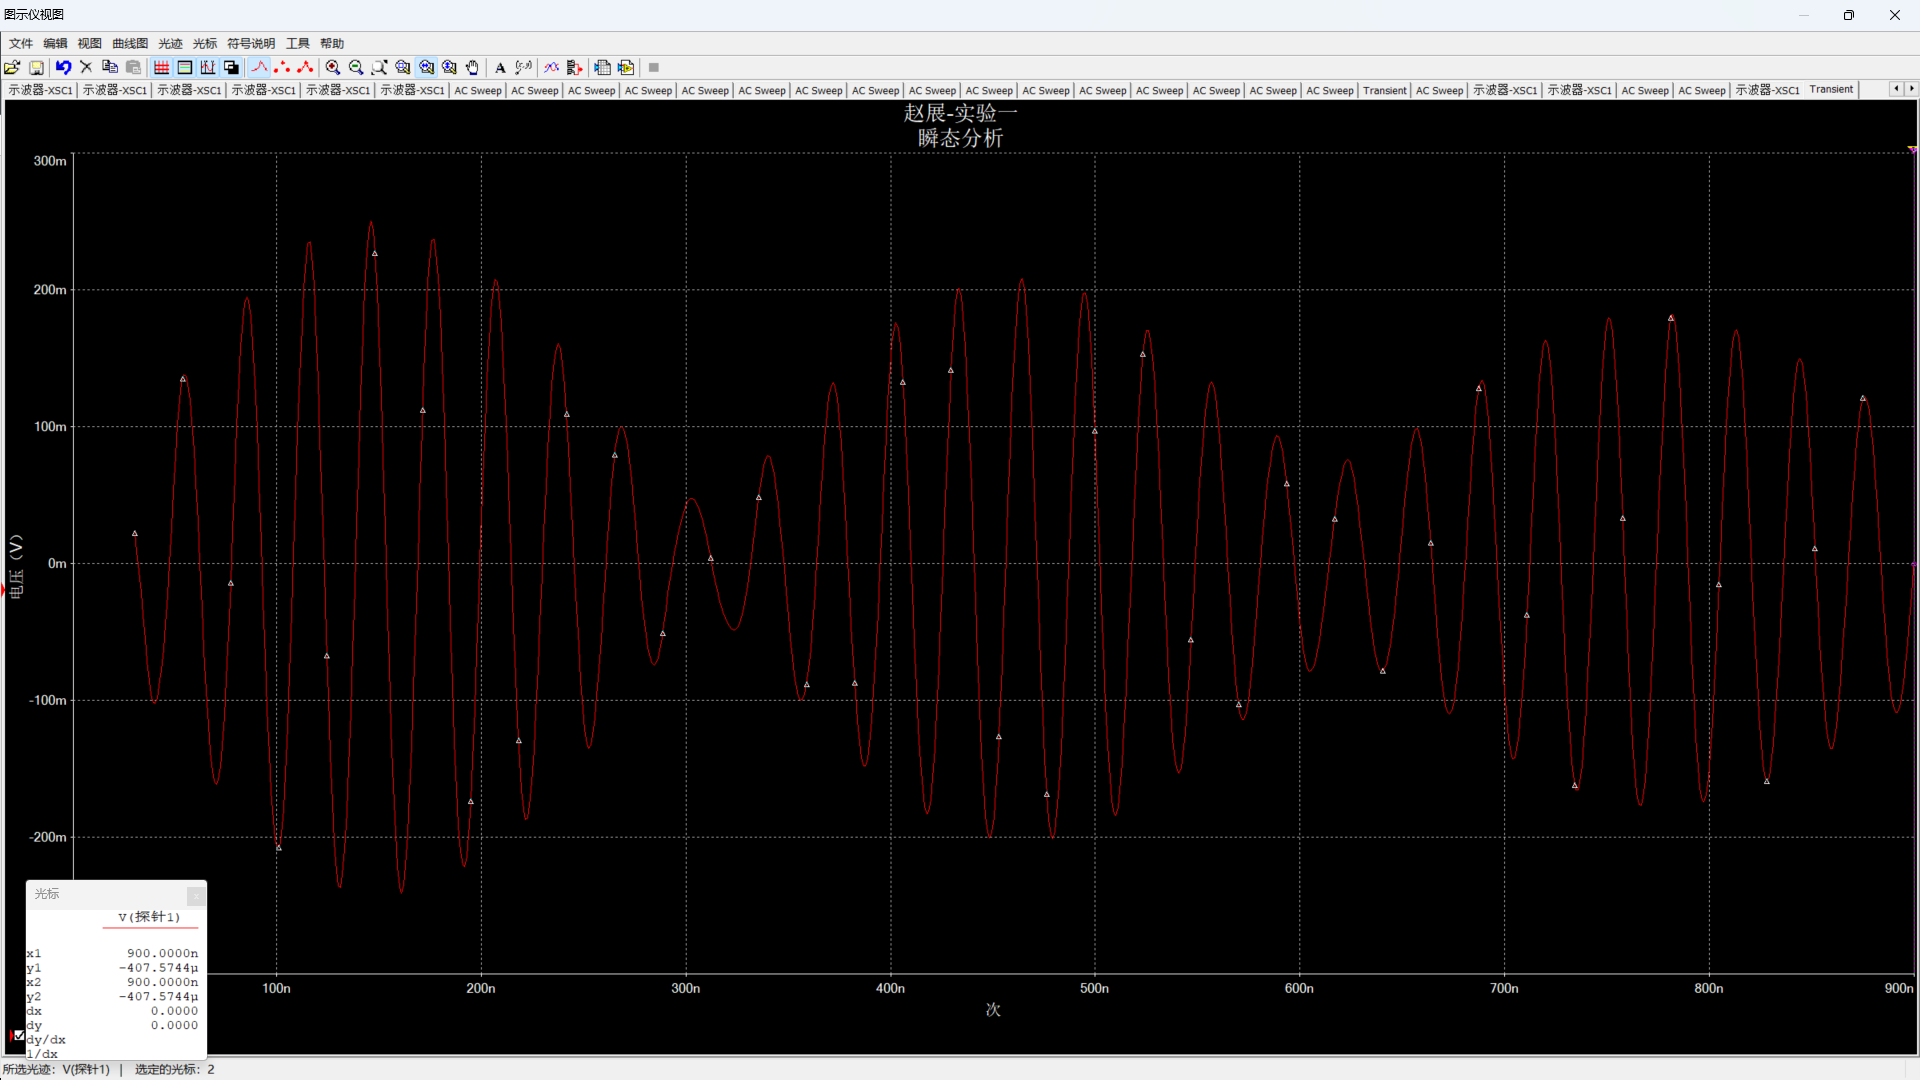
\includegraphics[width=0.8\linewidth]{multisim_transient_analysis.png}
    \caption{瞬态分析:电感/电容的电压}
    \label{img:multisim_transient_analysis}
\end{figure}
\subsection{频域特性}
\subsubsection{傅里叶分析-频谱}
分别对输入输出信号使用傅里叶分析,分别得到如图\ref{img:Fourier1},\ref{img:Fourier2}所示的频谱图。可以看出输入输出信号的交流成分的频率为50MHz,与自己设置的频率信号相符。
\begin{figure}[htbp]
    \centering
    \begin{minipage}[t]{0.49\textwidth}
        \centering
        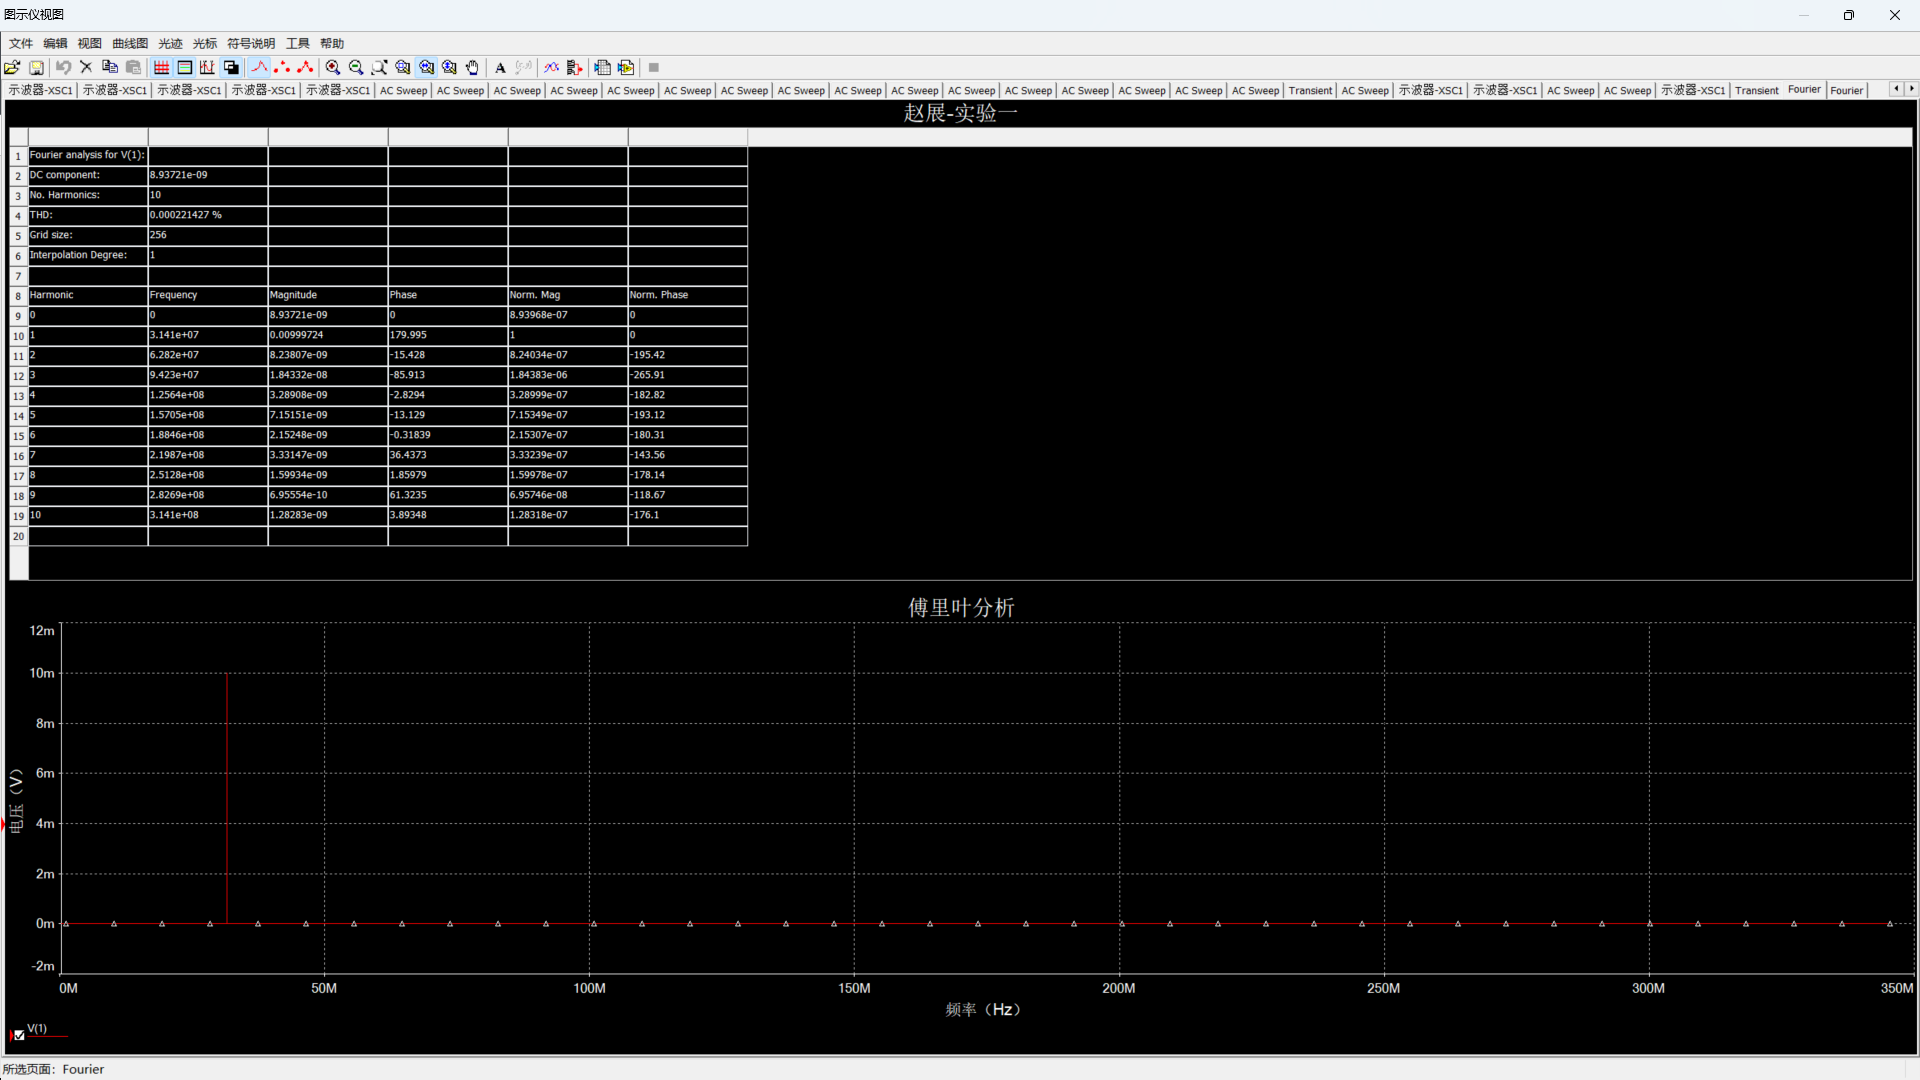
\includegraphics[width=0.7\linewidth]{Fourier_v1.png}
        \caption{输入频谱}
        \label{img:Fourier1}
    \end{minipage}
    \begin{minipage}[t]{0.49\textwidth}
        \centering
        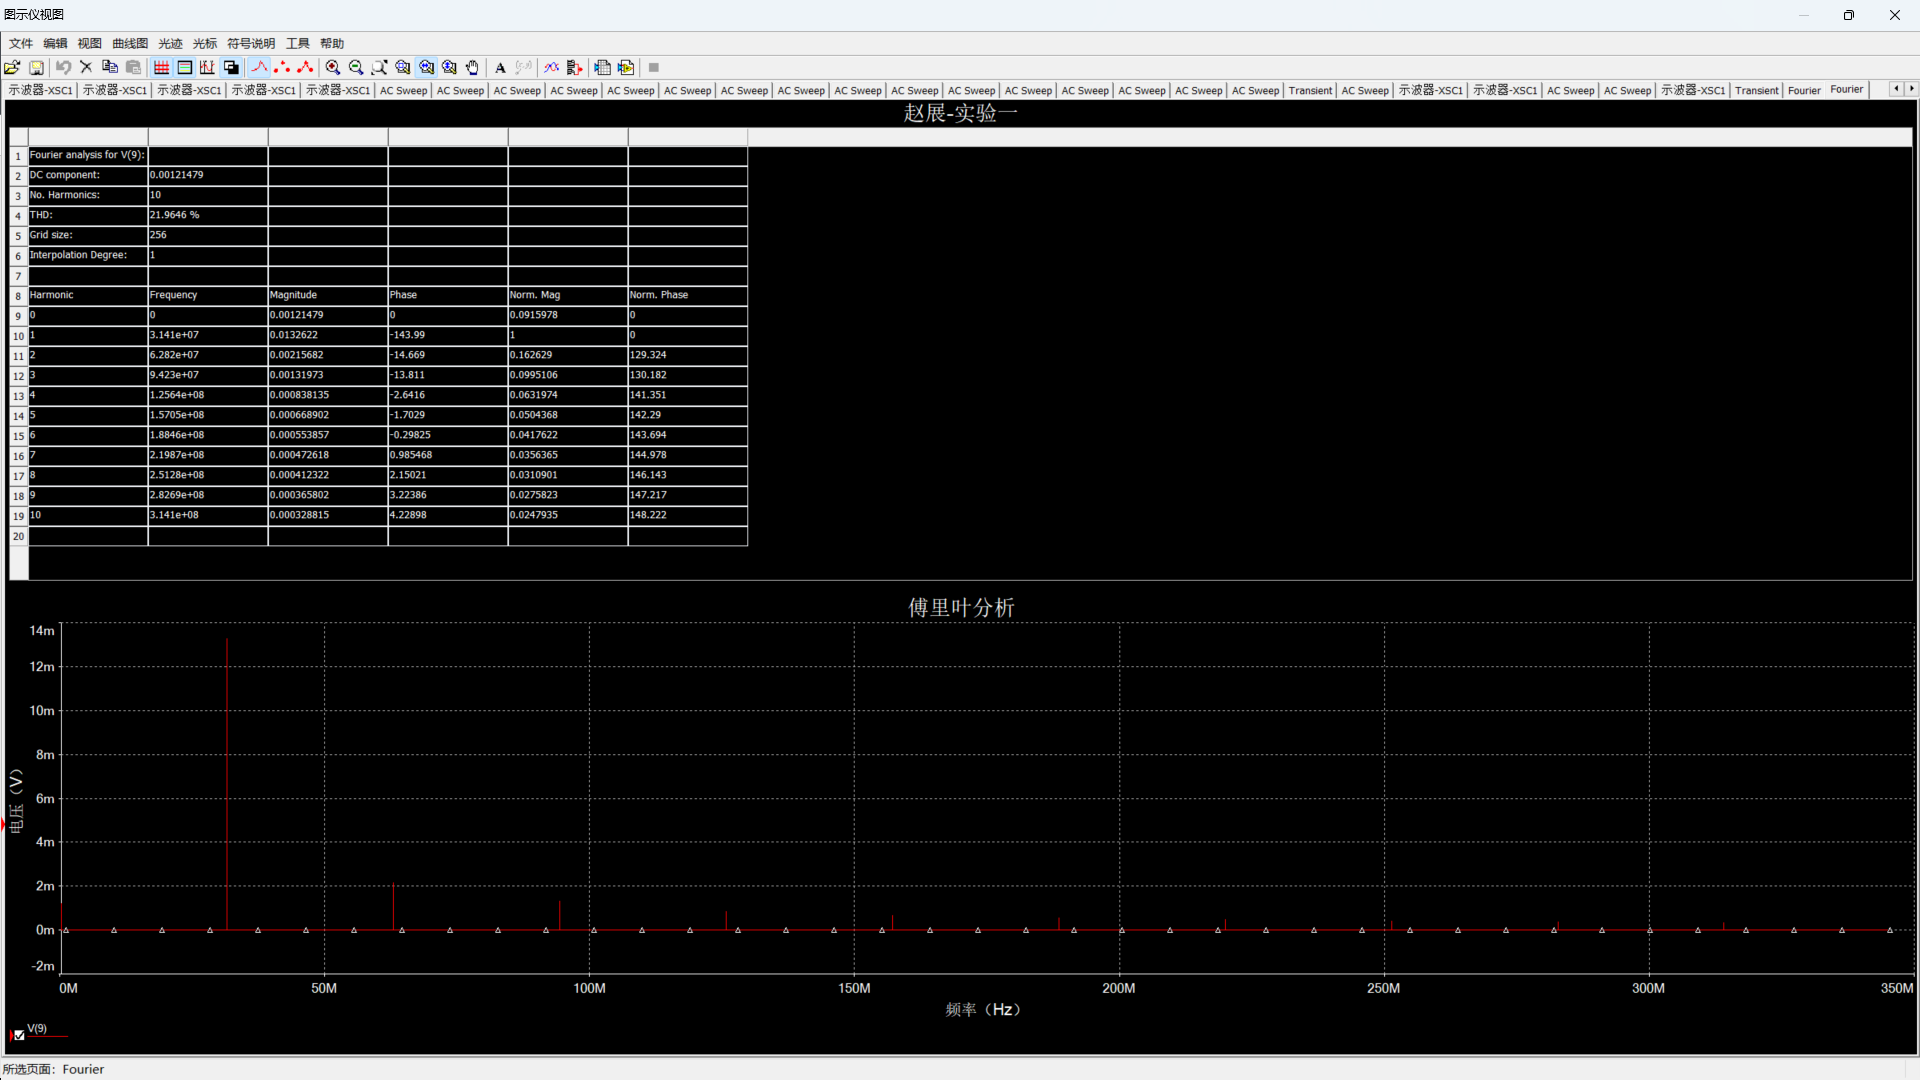
\includegraphics[width=0.7\linewidth]{Fourier_v5.png}
        \caption{输出频谱}
        \label{img:Fourier2}
    \end{minipage}
\end{figure}
\subsubsection{交流分析-幅相响应}
对该电路做交流分析,得到幅频响应和相频响应如图\ref{img:multisim_alternating_analyze}所示:
可以得到选频中心为34.7513MHz,最大增益为136.7117倍。
\begin{figure}[htbp]
    \centering
    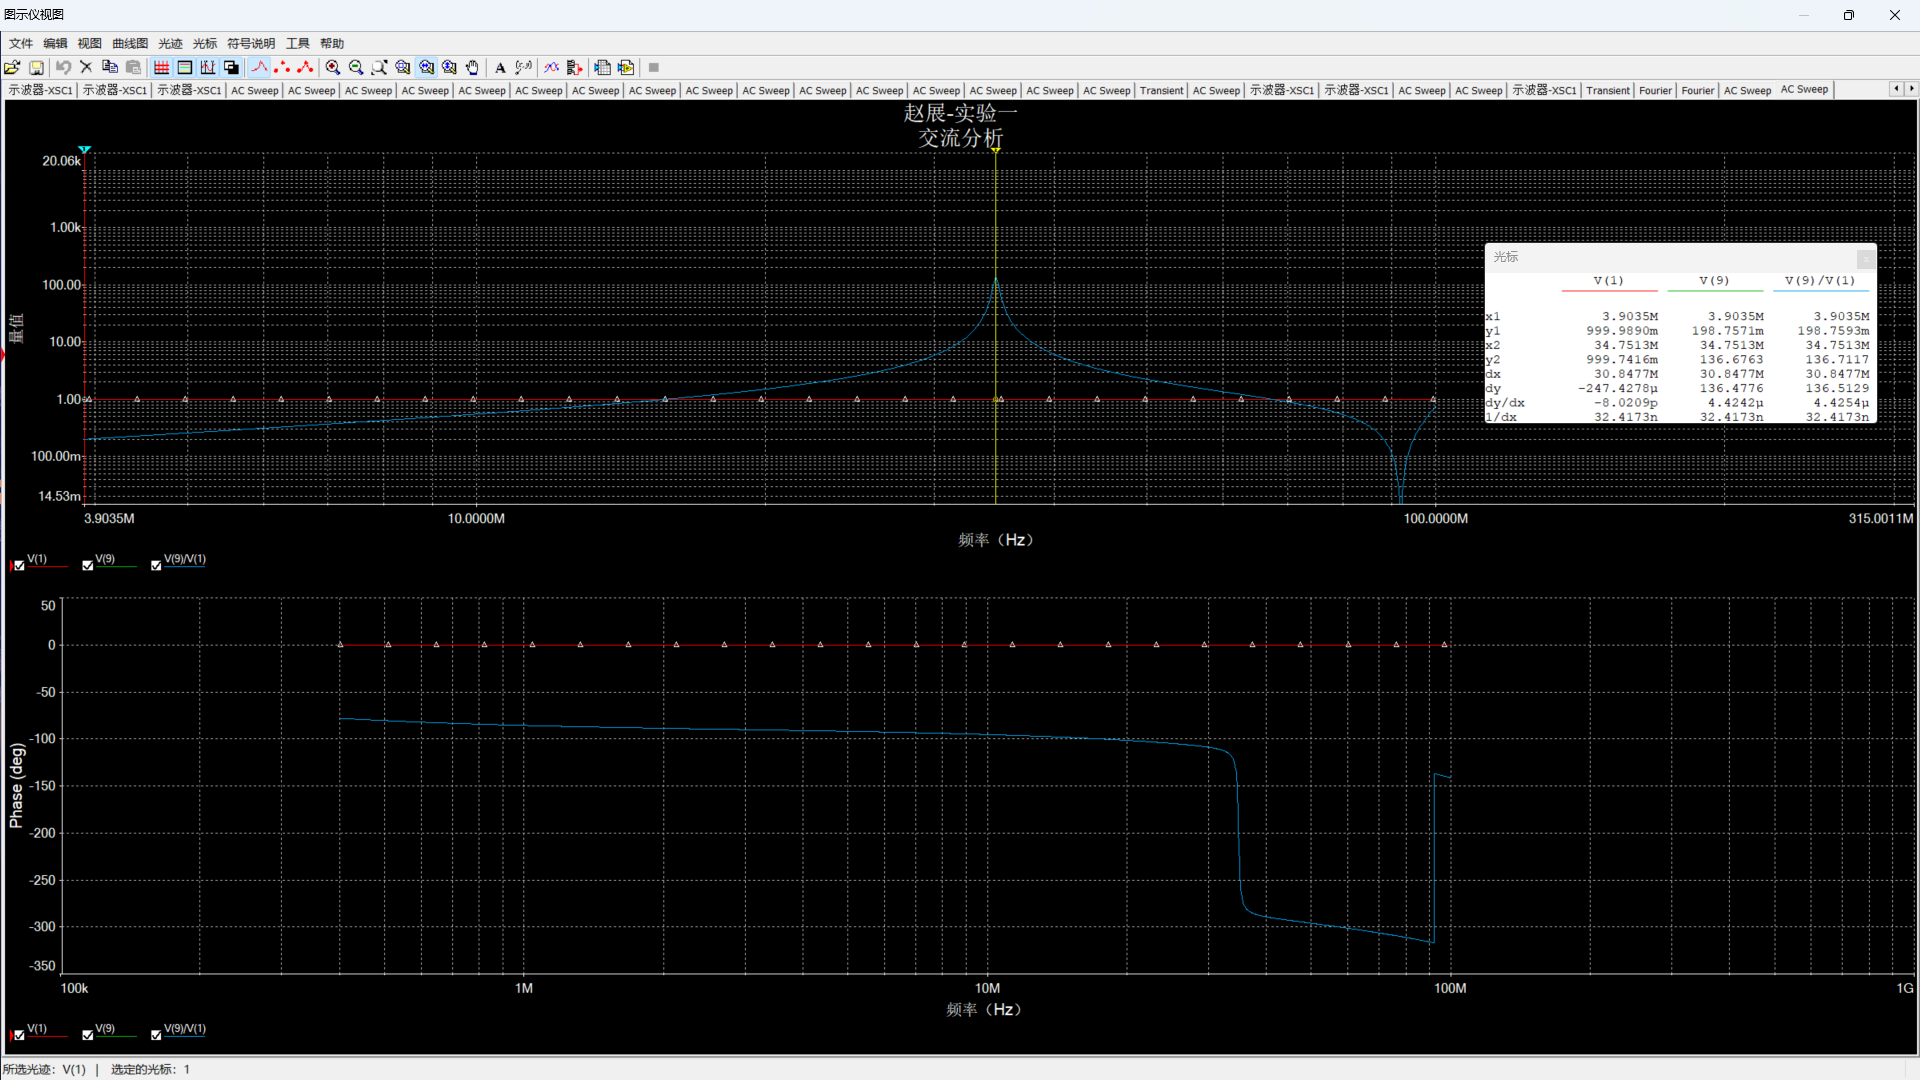
\includegraphics[width=0.8\linewidth]{multisim_alternating_analyze.png}
    \caption{交流分析:幅频特性曲线和相频特性曲线}
    \label{img:multisim_alternating_analyze}
\end{figure}
在幅频响应图上进行分析如图\ref{img:multisim_alternating_analysis}所示,
在最大增益的0.707倍处(136.7117*0.707=96.6552)
可以得到此时的频率为34.5538或34.9945MHz。
\begin{figure}[htbp]
    \centering
    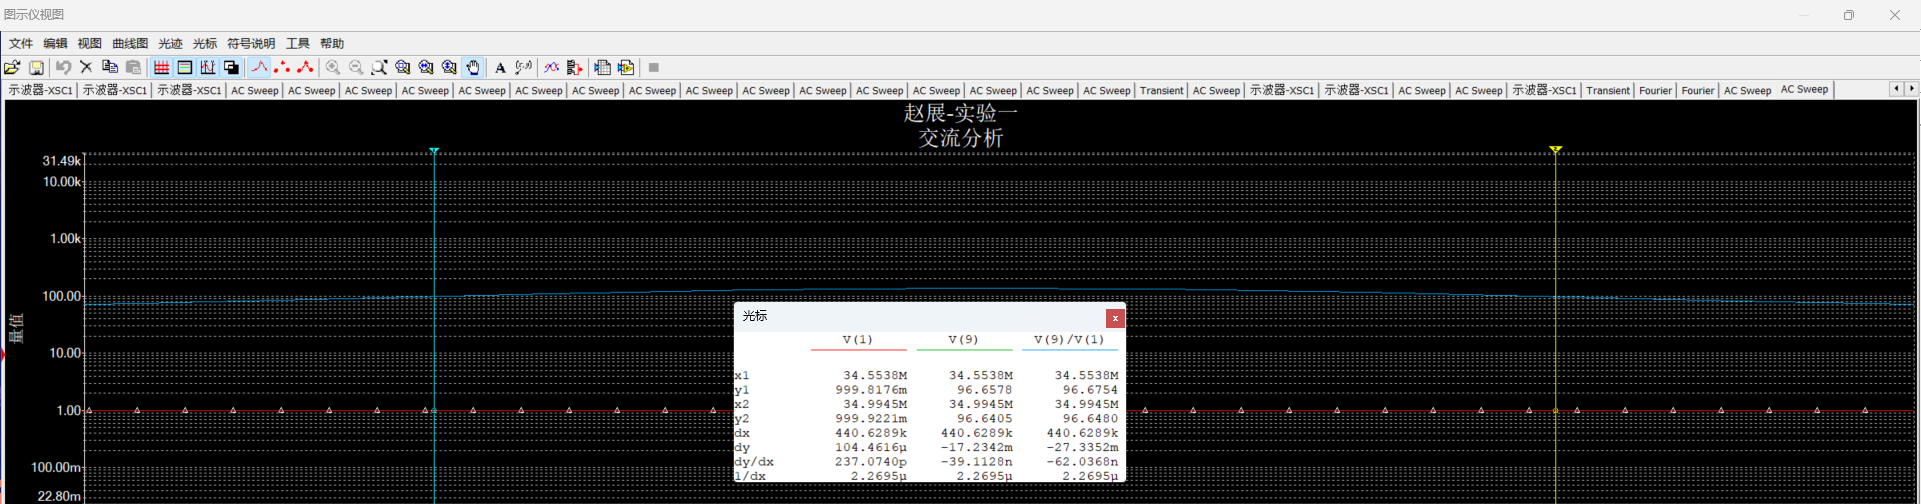
\includegraphics[width=0.8\linewidth]{multisim_alternating_analysis.png}
    \caption{交流分析:通频带分析}
    \label{img:multisim_alternating_analysis}
\end{figure}
所以通频带为:
$$
B=34.9945-34.5538=0.4407(MHz)
$$
\subsection{$Q_L,A_V,B$之间的关系}
\subsubsection{并入4K$\Omega$电阻}
在仿真电路中将4K$\Omega$电阻并入选频网络后,重新执行交流分析,得到的幅频响应如图\ref{img:multisim_alternating_analyze_R}所示
\begin{figure}[htbp]
    \centering
    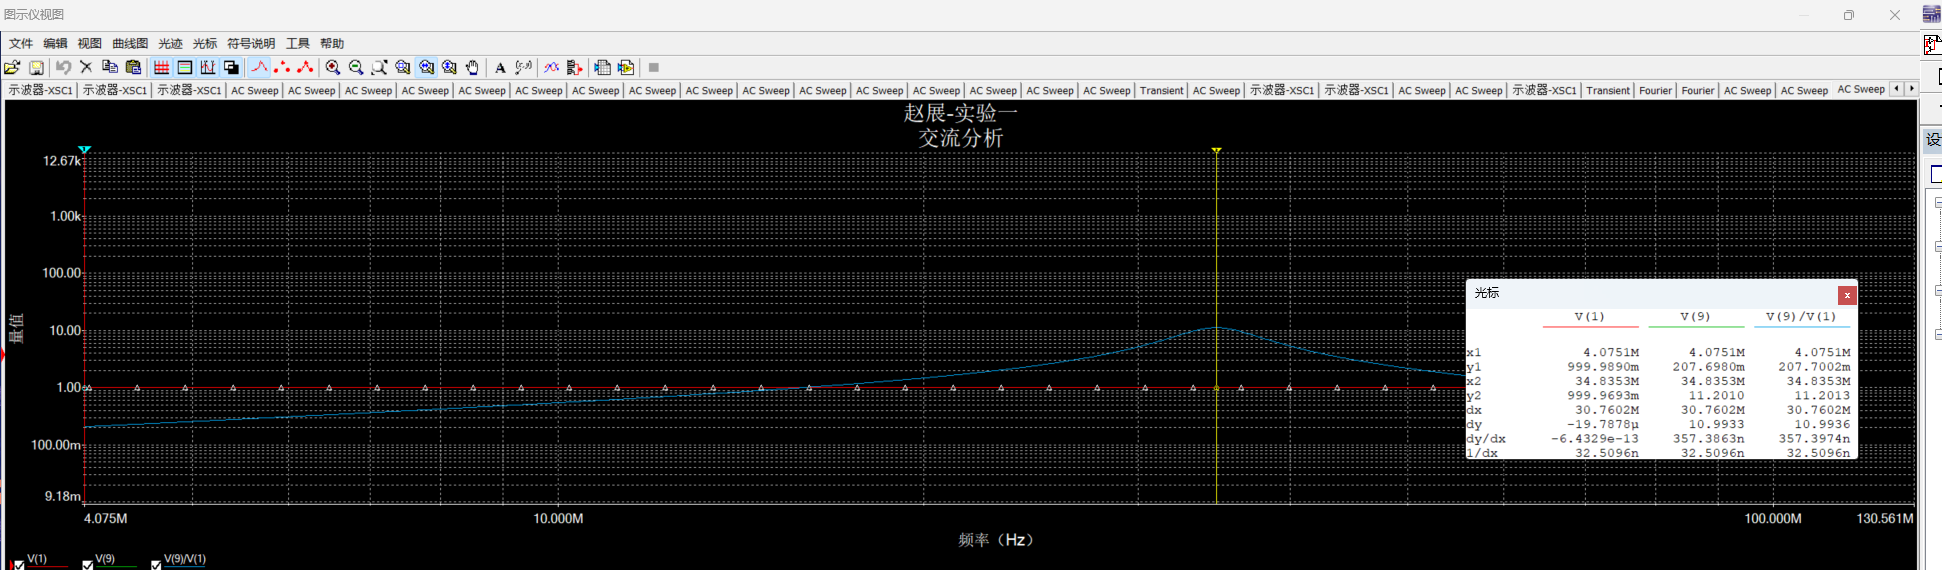
\includegraphics[width=0.8\linewidth]{multisim_alternating_analyze_R.png}
    \caption{交流分析:接入4K$\Omega$电阻后幅频分析}
    \label{img:multisim_alternating_analyze_R}
\end{figure}
可以看出接入4K$\Omega$电阻后,最大增益变为了11.2013倍,电压增益变小。
同样在其上分析通频带,将光标移动至最大增益的0.707倍处(11.2013*0.707=7.919),
如图所示可以算出通频带变为:
$$
B^{'}=37.5630-32.2212=5.3418(MHz)
$$
\begin{figure}[htbp]
    \centering
    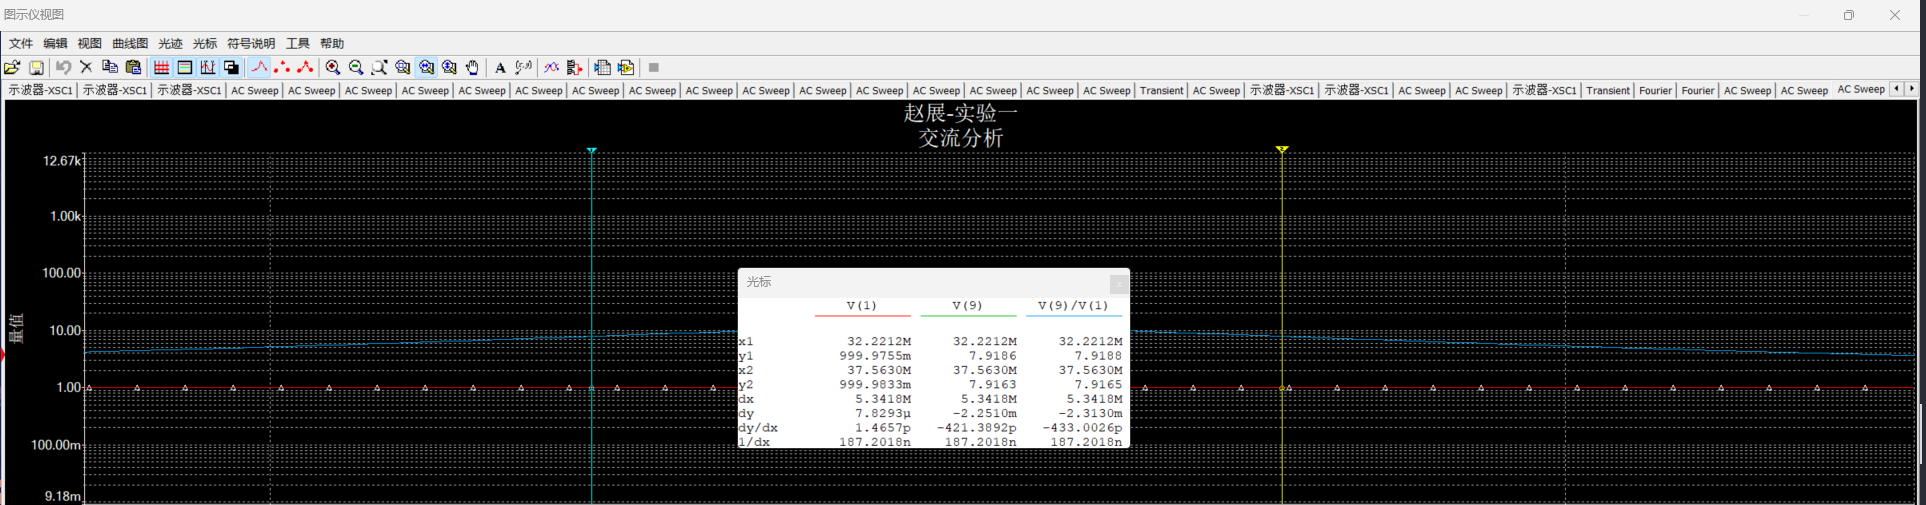
\includegraphics[width=0.8\linewidth]{multisim_alternating_analysis_R.png}
    \caption{交流分析:接入4K$\Omega$电阻后通频带分析}
    \label{img:multisim_alternating_analysis_R}
\end{figure}
可以看出,接入4K$\Omega$电阻后,通频带变宽,增益变小。
\subsubsection{$Q_L,A_V,B$关系验证}
接入4K$\Omega$电阻前:
$$
Q=\frac{f_0}{B}=\frac{34.7513}{0.4407}=78.8548
$$
$$
Q*B=34.7513*10^6
$$
$$
A_{V0}*B=60.2488*10^6
$$
接入4K$\Omega$电阻后:
$$
Q^{'}=\frac{f_0^{'}}{B^{'}}=\frac{34.8353}{5.3418}=6.5213
$$
$$
Q*B=34.8353*10^6
$$
$$
A_{V0}^{'}*B^{'}=59.8351*10^6
$$
可以看出Q*B为选频回路近似为常数,$A_{V0}*B$也近似为常数。
\section{实验小结}
本实验是通信电子线路的第一次实验,由于使用上的不熟练以及一开始电路参数选择错误,特别
是电容和电感的数量级选择不对,花费了一些时间调参。在认真研究了Multisim仿真软件和电路图
后重新选择的变压器以及参数,才把电路调通。学会了利用Multisim搭建电路、查看幅频和相频响
应的方法,为之后的实验打好基础。

本次报告撰写是第一次使用\LaTeX 进行排版,也花费了不少时间。
\end{document}
